% Raport v1.0 (F5.3 w ROADMAP.md). Liczby pochodzą z results/*.json i figures/*.md,
% które odtwarza `make figures`.
\documentclass[11pt,a4paper]{article}
\usepackage[T1]{fontenc}
\usepackage[utf8]{inputenc}
\usepackage{lmodern}
\usepackage[polish]{babel}
\usepackage[margin=2.3cm]{geometry}
\usepackage{microtype}
\usepackage{amsmath,amssymb}
\usepackage{graphicx}
\usepackage{booktabs,tabularx,array}
\usepackage[font=small,labelfont=bf]{caption}
\usepackage[hidelinks]{hyperref}
\graphicspath{{../figures/}}

\newcolumntype{L}{>{\raggedright\arraybackslash}X}
\newcommand{\QBER}{\mathrm{QBER}}

\title{Symulator BB84 z atakami:\\walidacja modelu, katalog ataków i~uwierzytelnianie postkwantowe}
\author{Shertie}
\date{wersja 1.0, \today}

\begin{document}
\maketitle

\begin{abstract}
Opisujemy symulator Monte Carlo protokołu BB84 na poziomie pojedynczych impulsów: od źródła słabych impulsów koherentnych przez światłowód i detektory SPAD do klucza końcowego po korekcji błędów i wzmacnianiu prywatności. Model z parametrami eksperymentu GYS odtwarza wzory Ma i in.\ (2005) dla zysku, QBER i stopy klucza, a wyniki krzyżowo zgadzają się z niezależną implementacją \texttt{qkd}. Na tym torze wykonujemy pięć ataków (intercept-resend, oślepianie detektorów, PNS, optymalny atak indywidualny, man-in-the-middle) i porządkujemy je w mapę ,,atak $\to$ złamane założenie dowodu $\to$ obrona $\to$ metryka''. Ostatnia część porównuje uwierzytelnianie kanału klasycznego kluczem współdzielonym (Wegman--Carter) i podpisem ML-DSA (FIPS~204) oraz zestawia QKD z ML-KEM w kilku modelach zagrożeń.
\end{abstract}

\section{Wstęp}

Dowody bezpieczeństwa QKD \cite{shor2000simple,gllp2004,scarani2009security} opierają się na założeniach o urządzeniach i o kanale klasycznym. Praktyczne ataki \cite{brassard2000limitations,lydersen2010hacking,zhao2008quantum,gisin2006trojan} nie łamią samego wzoru na długość klucza, tylko któreś z tych założeń, często bez śladu w QBER \cite{xu2020secure}. Celem projektu jest pokazanie tego na jednym, zwalidowanym modelu: każdy atak jest \emph{wykonywany} na impulsach, a nie wyceniany wzorem, a każdy wynik Monte Carlo porównujemy ze wzorem albo z liczbą z publikacji.

Istnieją narzędzia o podobnym zakresie. Najbliższe jest \texttt{qkd} (PyPI), które odtwarza Ma i in.\ dla GYS i wycenia część tych samych ataków w formie zamkniętej, bez symulacji impulsów. Używamy go jako niezależnej wyroczni w testach krzyżowych. Uwierzytelnianie QKD podpisami postkwantowymi pokazano już eksperymentalnie \cite{wang2021experimental}; nowością nie jest więc sama idea, tylko zestawienie w jednym symulatorze, kiedy takie uwierzytelnianie chroni klucz, a kiedy nie.

Wkład projektu:
(i) tor Monte Carlo BB84 z WCP, decoy, Cascade, haszem Toeplitza i skończonym kluczem, zgodny ze wzorami na 0--150~km;
(ii) ataki 1, 2, 3, 6 i 7 z obronami i krzywymi ROC;
(iii) mapa ataków na założenia dowodu;
(iv) porównanie Wegmana--Cartera, ML-DSA i hybrydy oraz tabela modeli zagrożeń QKD wobec ML-KEM.

\section{Model}

\subsection{Źródło, kanał, detektory}

Alice wysyła impulsy koherentne o średniej liczbie fotonów $\mu$ (rozkład Poissona), kodując bit w jednej z dwóch baz polaryzacji. Kanał to światłowód o tłumieniu $\alpha = 0{,}21$~dB/km z błędem optyki $e_d = 3{,}3\%$, a Bob ma dwa detektory SPAD o łącznej sprawności $\eta_{\mathrm{Bob}} = 4{,}5\%$ i tle $Y_0 = 1{,}7\cdot 10^{-6}$ na bramkę. To parametry eksperymentu GYS \cite{gobby2004qkd} w opracowaniu Ma i in.\ \cite{ma2005practical}, z $f_{\mathrm{EC}} = 1{,}22$ i $\mu = 0{,}48$, $\nu = 0{,}05$ dla decoy vacuum+weak \cite{lo2005decoy}. Podwójne kliknięcia dostają losowy bit, zgodnie z modelem squashing \cite{beaudry2008squashing}.

Symulacja ma dwie warstwy. Warstwa bitów zapisuje każdy impuls (bit, bazę, intensywność, liczbę fotonów, kąt polaryzacji, moc) i kończy się kluczem po siftingu. Warstwa liczników przetwarza te same modele w paczkach i zwraca tylko zliczenia, co pozwala na $10^9$ impulsów na punkt. Losowość pochodzi z osobnych strumieni (Alice, Bob, natura, Ewa, kanał publiczny) wyprowadzonych z jednego ziarna, więc każdy wykres jest deterministyczny i można go liczyć równolegle.

Atak to jeden z trzech typów zaczepów: na impulsach w punkcie światłowodu, na detektorach albo na wiadomościach kanału klasycznego. Ewa ma własny strumień losowy i dziennik tego, co wie.

\subsection{Postprocessing}

Po siftingu Alice i Bob ujawniają losową próbkę (10\%) i estymują z niej QBER. Korekcję błędów robi Cascade z czterema przebiegami \cite{brassard1994cascade,martinezmateo2015cascade}, a każda ujawniona parzystość trafia do licznika wycieku $\mathrm{leak}_{\mathrm{EC}}$. Zgodność kluczy sprawdza hasz uniwersalny, a wzmacnianie prywatności to mnożenie przez losową macierz Toeplitza. Długość klucza liczymy wzorem GLLP z granicami decoy. Wiedzę pasywnej Ewy mierzymy dokładnie: ujawnione parzystości i wiersze macierzy Toeplitza to funkcje liniowe klucza nad GF(2), więc liczba bitów klucza końcowego znanych Ewie to wymiar przecięcia ich rozpięć.

\subsection{Implementacja i testy}

Kod to Python i numpy, sprawdzany \texttt{mypy --strict}. Testy: 375 szybkich (jednostkowe, regresji ze ,,złotymi wartościami'', własności przez \texttt{hypothesis}, krzyżowe z \texttt{qkd}) i 55 wolnych: statystyczne, które porównują Monte Carlo ze wzorem przez $z$-score przy stałych ziarnach ($|z| < 4$), oraz krzyżowe z QuTiP. Pokrycie gałęzi rdzenia szybkimi testami: 95\%. Fragmenty kwantowe ataku 6 weryfikuje niezależnie QuTiP. Każdy z dziesięciu eksperymentów kończy się błędem, jeśli wynik wyjdzie poza tolerancję, a całość odtwarza \texttt{make figures}.

\section{Walidacja}

\begin{figure}[t]
  \centering
  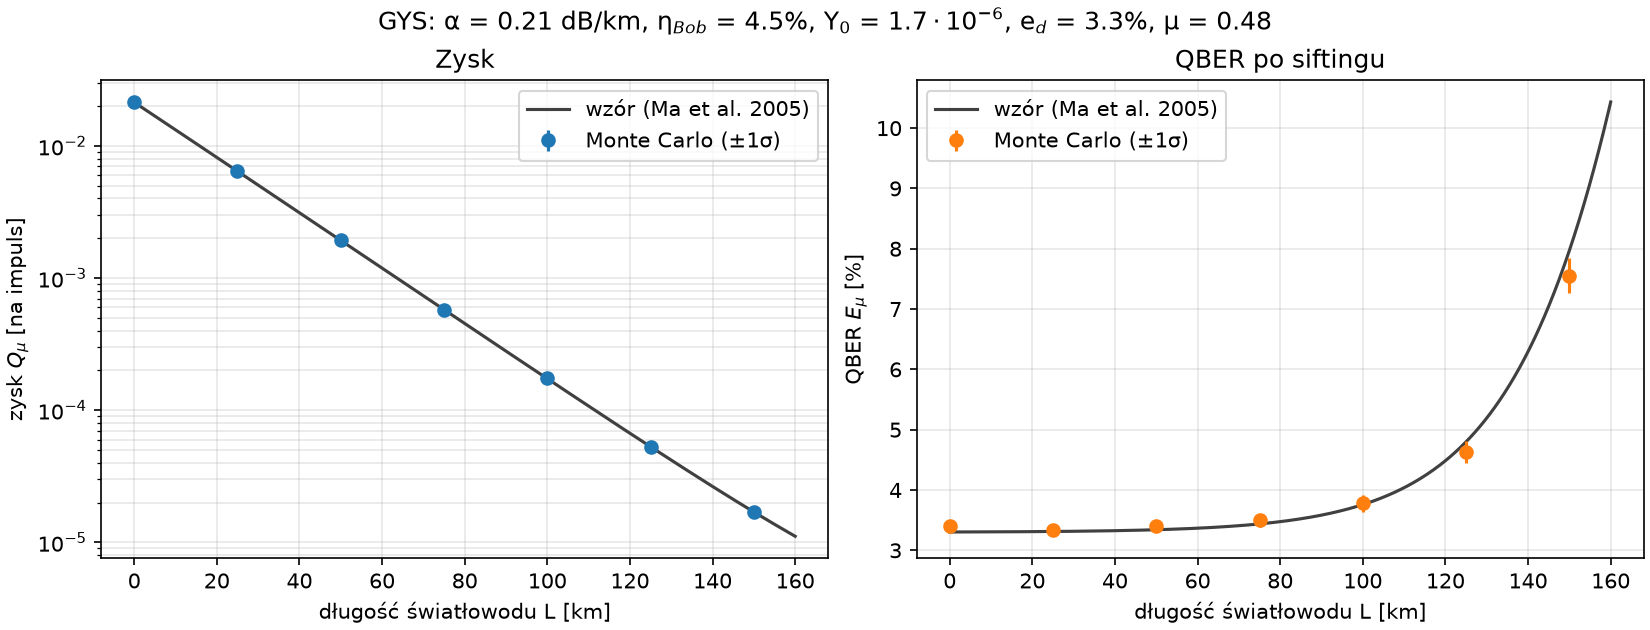
\includegraphics[width=\linewidth]{e01_gain_qber_vs_L}
  \caption{Zysk i QBER w funkcji długości światłowodu: Monte Carlo (punkty, do $10^9$ impulsów) na tle wzorów Ma i in.\ \cite{ma2005practical} dla GYS. Wszystkie punkty w granicach $|z| < 1{,}8$.}
  \label{fig:e01}
\end{figure}

Bez ataku zysk i QBER z Monte Carlo zgadzają się ze wzorami na całym zakresie 0--150~km (rys.~\ref{fig:e01}). Tabela~\ref{tab:control} zbiera wartości kontrolne z planu projektu: liczby z literatury, nasze przeliczenie i wynik niezależnej implementacji \texttt{qkd}~0.2.0.

\begin{table}[t]
  \centering
  \caption{Wartości kontrolne. ,,Model'' to nasza implementacja wzorów i Monte Carlo.}
  \label{tab:control}
  \small
  \begin{tabularx}{\linewidth}{L l l l}
    \toprule
    Wielkość & Literatura & Model & \texttt{qkd} \\
    \midrule
    QBER, pełny intercept-resend (25~km) & $1/4 + e_d/2 = 26{,}65\%$ & 26,5--26,8\% (MC) & --- \\
    Próg Shora--Preskilla $1 - 2h(Q) = 0$ & $Q^* = 0{,}110028$ & $0{,}110028$ & --- \\
    Przecięcie $I_{AB} = I_{AE}$ (Fuchs) & $D^* = 0{,}146447$ & $0{,}146447$ (MC $\pm 3\sigma$) & --- \\
    $L_{\max}$, nieskończenie wiele decoy & 142,05~km & 142,01~km & 142,01~km \\
    $L_{\max}$, vacuum+weak & 140,55~km & 140,62~km & 140,62~km \\
    Odchylenie $Y_1^L$ / $e_1^U$ przy 40~km & 3,5\% / 16,8\% & zgodne & 3,51\% / 16,78\% \\
    $L_{\max}$, GLLP bez decoy & --- & $\approx 40$~km & 40,21~km \\
    Sprawność Cascade, $Q = 0{,}5$--$8\%$ & 1,1--1,2 & 1,106--1,191 & --- \\
    \bottomrule
  \end{tabularx}
\end{table}

\section{Ataki i obrony}

Tabela~\ref{tab:map} to centralny wynik projektu. Każdy atak, który nie podnosi QBER, łamie jedno z założeń dowodu, a obrona przywraca to założenie albo wykrywa jego złamanie. Plan projektu przewidywał to dla ataków 2, 4, 5, 7 i 8; wyniki dodają do listy PNS, który przy niezmienionym QBER i zysku łamie założenie o znanym rozkładzie liczby fotonów.

\begin{table}[t]
  \centering
  \caption{Mapa ataków v1.0. Z1: rozkład liczby fotonów uwzględniony w długości klucza; Z3: detektor jednofotonowy o sprawności niezależnej od bitu i czasu; Z5a: kanał klasyczny uwierzytelniony w trakcie sesji; Z5b: klucze publiczne autentyczne; Z7: Ewa ograniczona tylko fizyką; Z8: estymacja ze skończonej próbki z jawnym $\varepsilon$.}
  \label{tab:map}
  \small
  \begin{tabularx}{\linewidth}{>{\raggedright\arraybackslash}p{2.6cm} >{\raggedright\arraybackslash}p{2.6cm} >{\raggedright\arraybackslash}p{3.2cm} L}
    \toprule
    Atak & Złamane założenie & Obrona & Metryka (wynik) \\
    \midrule
    1. Intercept-resend & żadne; przy małej próbce Z8 & próg QBER 11\%, skończony klucz & QBER 26,5\% przy pełnym ataku; przechwycenie 4\% impulsów wykryte w 23\% sesji przy próbce 1000 bitów \\
    2. Oślepianie detektorów & Z3 & losowe tłumienie 3~dB w 10\% bramek; monitor mocy & QBER i zysk bez zmian, Ewa zna 100\% klucza; test tłumienia $z \approx -35$, AUC $= 1$ od $3\cdot 10^4$ bramek \\
    3. PNS & Z1 & stany decoy & od 32,8~km Ewa zna 98--100\% klucza; spójność decoy $z$ od $-69$ do $-10$, AUC $= 1$ \\
    6. Optymalny atak indywidualny & Z7 (granica indywidualna to nie granica ogólna) & próg Shora--Preskilla 11,00\% & $I_{AB} = I_{AE}$ przy $D^* = 14{,}64\%$; numpy i QuTiP zgodne do $10^{-12}$ \\
    7. Man-in-the-middle & Z5a & Wegman--Carter & przerwanie przy pierwszym tagu Ewy; fałszerstwo $1/p \approx 2^{-61}$ \\
    7$'$. MITM przy ML-DSA & Z5a w trakcie sesji, Z5b & hybryda WC + ML-DSA, odcisk klucza & podpis złamany na żywo lub podmieniony klucz: MITM udany; hybryda wykrywa \\
    \bottomrule
  \end{tabularx}
\end{table}

\subsection{Intercept-resend}

Ewa mierzy ułamek $p$ impulsów w losowej bazie i wysyła Bobowi stan odpowiadający wynikowi. Przy pełnym ataku na 25~km QBER rośnie do 26,5--26,8\%, zgodnie z $1/4 + e_d/2$ (rys.~\ref{fig:e04}). Ewa tuż za Alice zdradza się też spadkiem zysku o 20\%, bo zamiast impulsu o średnio $\mu$ fotonach wysyła jeden foton, a z impulsów pustych w jej punkcie nic. Dla źródła WCP QBER$(p)$ leży poniżej prostej $e_d + p(1/4 - e_d/2)$, dokładnej tylko dla $p \in \{0, 1\}$, bo impulsy przechwycone są wykrywane rzadziej niż pozostałe.

\begin{figure}[t]
  \centering
  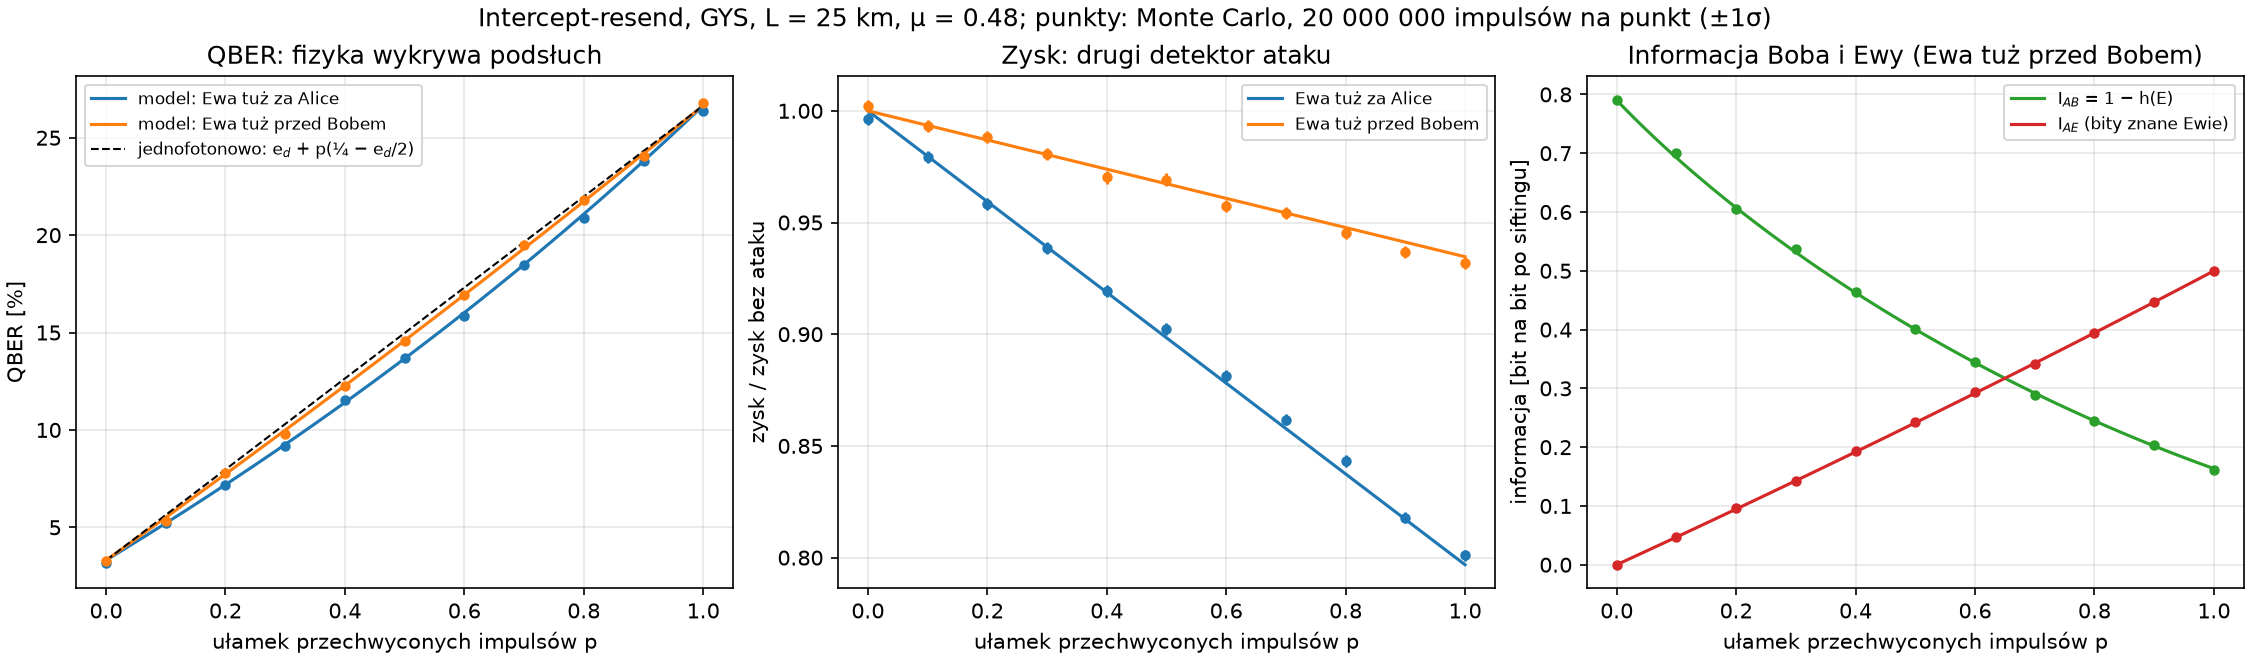
\includegraphics[width=\linewidth]{e04_intercept_resend}
  \caption{Intercept-resend przy 25~km: QBER, zysk i wiedza Ewy w funkcji ułamka przechwyconych impulsów $p$ i położenia Ewy.}
  \label{fig:e04}
\end{figure}

\subsection{Oślepianie detektorów}

Ewa oślepia detektory Boba ciągłym światłem (1,08~mW) i w każdej bramce wyzwala detektor odpowiadający jej wynikowi jasnym impulsem, jak w ataku Lydersena i in.\ na Clavis2 \cite{lydersen2010hacking}. Detektor ma tryb liniowy z progami $P_{\mathrm{never}}$ i $P_{\mathrm{always}}$ z tej pracy. Skalibrowana Ewa (impuls 950--1300~µW i kompensacja obrotu polaryzacji) zostawia QBER i zysk bez zmian, a zna cały klucz (rys.~\ref{fig:e05}). Losowe tłumienie 3~dB w 10\% bramek wykrywa ją z $z \approx -35$: po stłumieniu impuls wyzwalający spada poniżej progu i kliknięć brakuje. Monitor mocy wykrywa samo oślepianie bez trudu (AUC $= 1$ przy 1,08~mW), a gubi się tylko przy mocach rzędu µW, które detektora nie oślepiają. Żadna moc impulsu nie przechodzi jednocześnie testu QBER i testu tłumienia.

\begin{figure}[t]
  \centering
  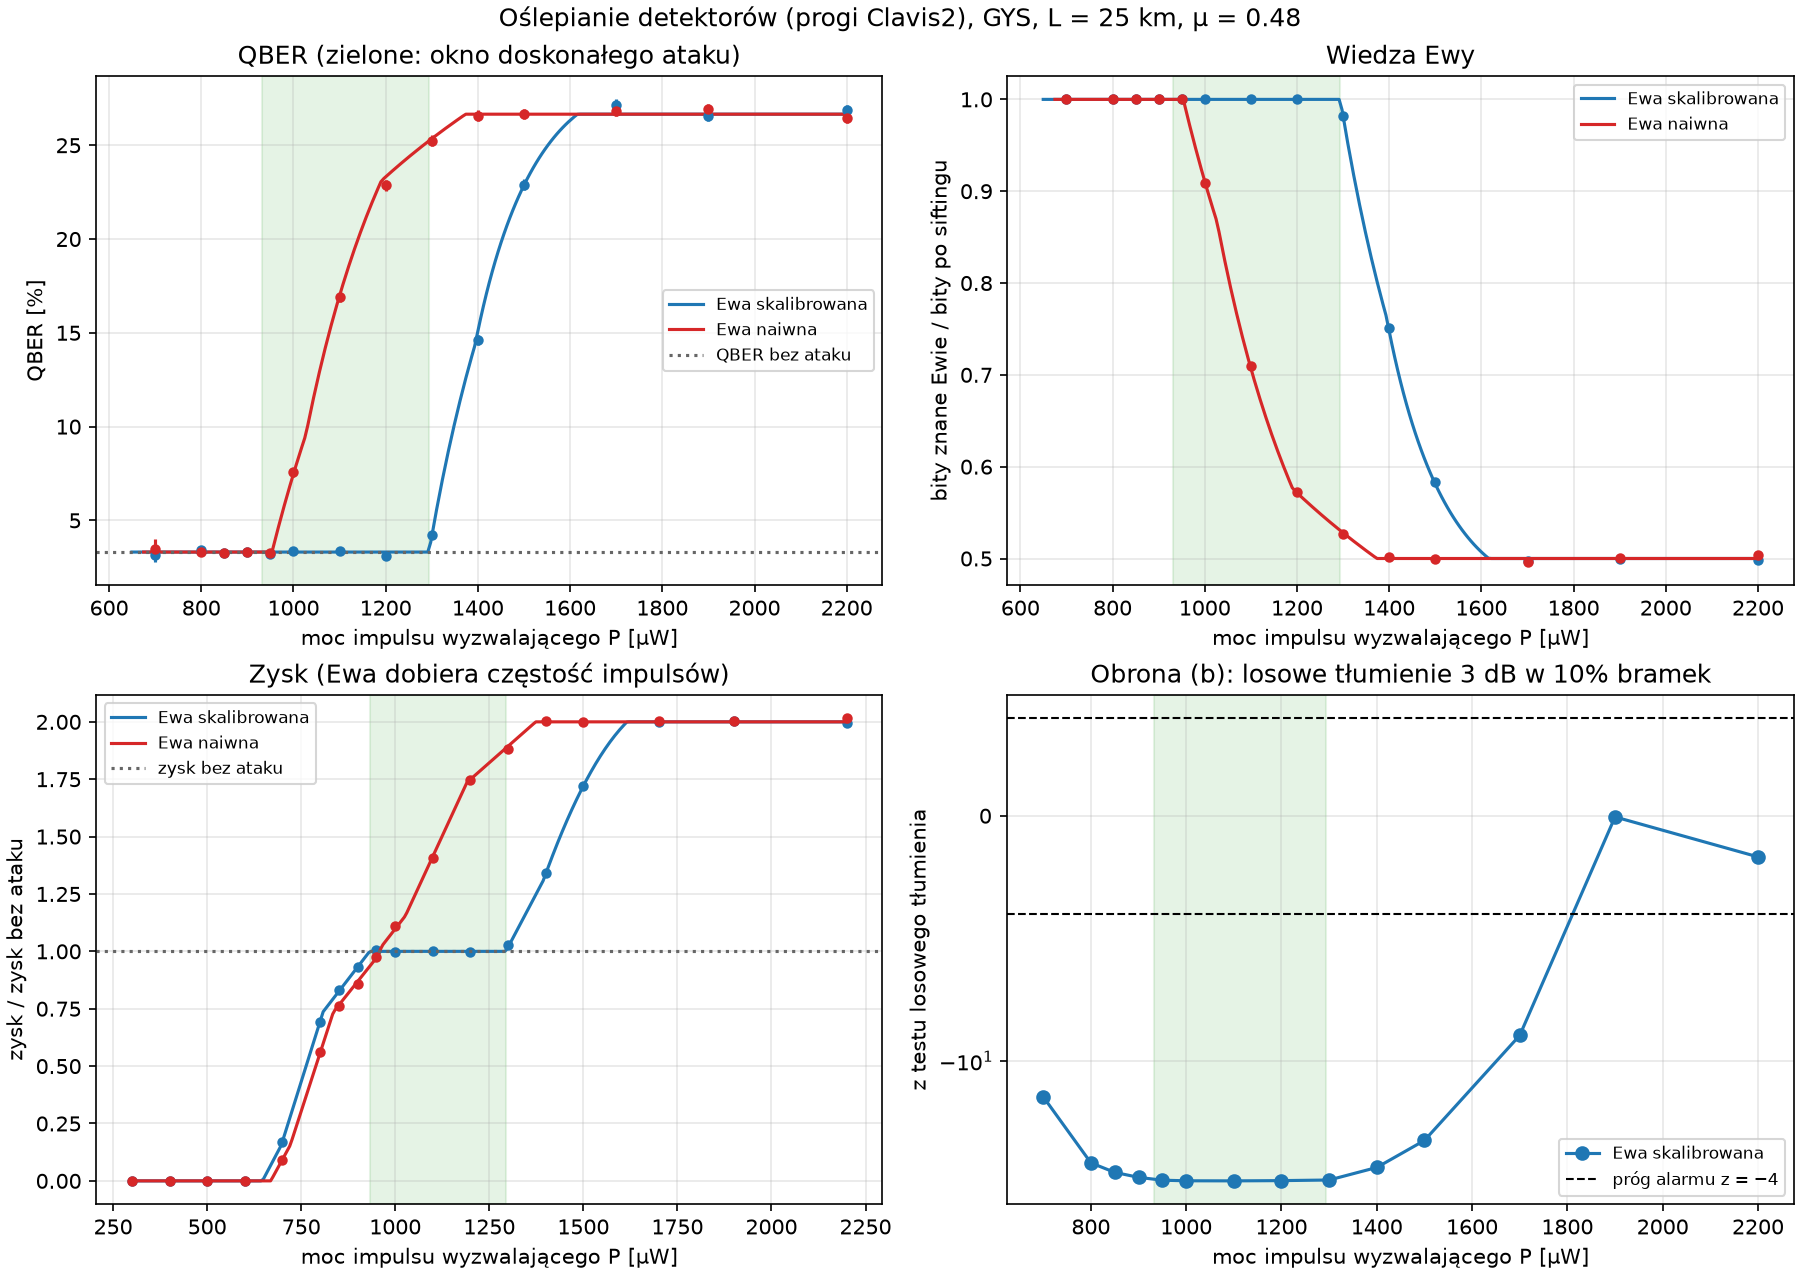
\includegraphics[width=0.78\linewidth]{e05_blinding}
  \caption{Oślepianie detektorów: QBER, zysk i wiedza Ewy w funkcji mocy impulsu wyzwalającego oraz wynik testu losowego tłumienia.}
  \label{fig:e05}
\end{figure}

\subsection{Photon-number splitting i stany decoy}

Ewa mierzy liczbę fotonów bez niszczenia polaryzacji, blokuje część impulsów jednofotonowych, a z wielofotonowych zatrzymuje foton i odczytuje go po ujawnieniu baz \cite{brassard2000limitations}. Od odległości krytycznej 32,8~km może zablokować tyle impulsów jednofotonowych, by przy bezstratnej linii do Boba zachować jego zysk i QBER, a zna wtedy 98--100\% klucza. Rachunek naiwny (,,każda detekcja jest jednofotonowa'') daje dodatnią stopę, choć klucz jest w całości u Ewy. Z decoy Ewa nie może zachować zysków obu intensywności naraz: dolna granica $Y_1$ spada do zera, stopa staje się ujemna i protokół się przerywa. Test spójności zysków sygnału i decoy daje $z$ od $-69$ (40~km) do $-10$ (120~km) przy $|z| < 1{,}1$ bez ataku. Rys.~\ref{fig:e06} pokazuje R(L): GLLP bez decoy kończy się przy około 40~km, decoy vacuum+weak przy 140,6~km.

\begin{figure}[t]
  \centering
  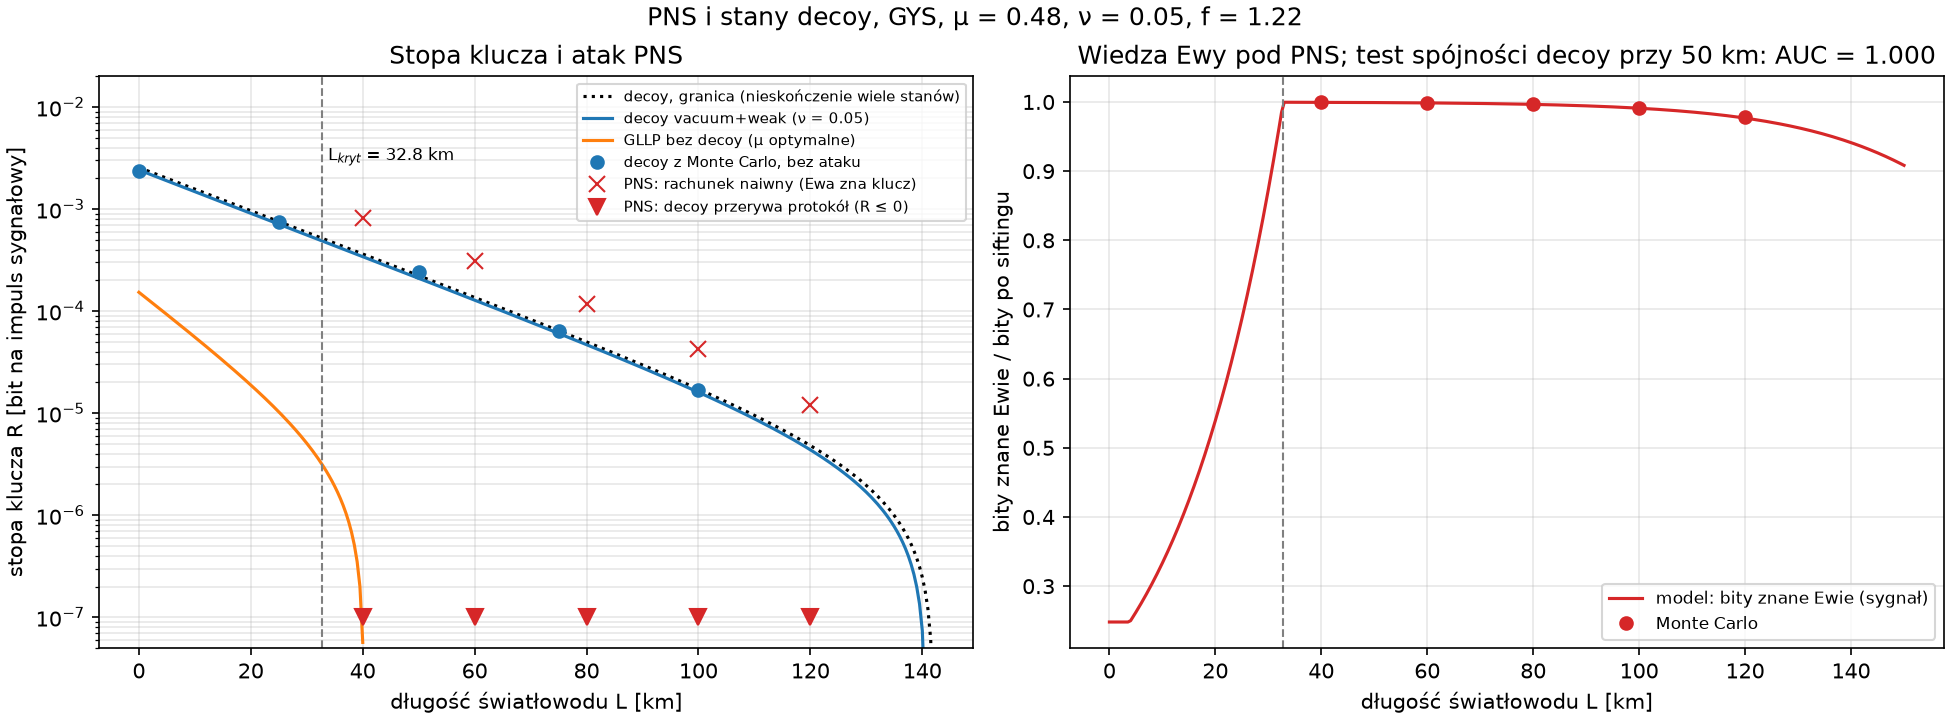
\includegraphics[width=\linewidth]{e06_decoy_pns}
  \caption{Stopa klucza R(L) dla GYS: GLLP bez decoy, decoy vacuum+weak i granica nieskończenie wielu decoy, z estymatą decoy z Monte Carlo (punkty), oraz wiedza Ewy przy ataku PNS.}
  \label{fig:e06}
\end{figure}

\subsection{Optymalny atak indywidualny}

Optymalny atak indywidualny na BB84 \cite{fuchs1997optimal} realizujemy jako kloner fazowo-kowariantny: częściowa zamiana stanów $|01\rangle$ i $|10\rangle$ kubitu i ancilli o kąt $\eta$, w układzie obróconym tak, by bazy Z i X leżały na równiku. Daje on błąd Boba $D = \sin^2(\eta/2)$ i błąd Ewy $1/2 - \sqrt{D(1-D)}$, czyli granicę Fuchsa, dla wszystkich czterech stanów. QuTiP buduje tę operację niezależnie z generatora; unitarność, wierności i prawdopodobieństwa wyników zgadzają się do $10^{-12}$. Monte Carlo daje $I_{AB} = I_{AE}$ przy $D^* = 14{,}64\%$ (rys.~\ref{fig:e08}). Próg Shora--Preskilla 11,00\% jest niższy, bo obejmuje ataki koherentne; klucz z QBER między tymi progami byłby bezpieczny tylko wobec ataków indywidualnych.

\begin{figure}[t]
  \centering
  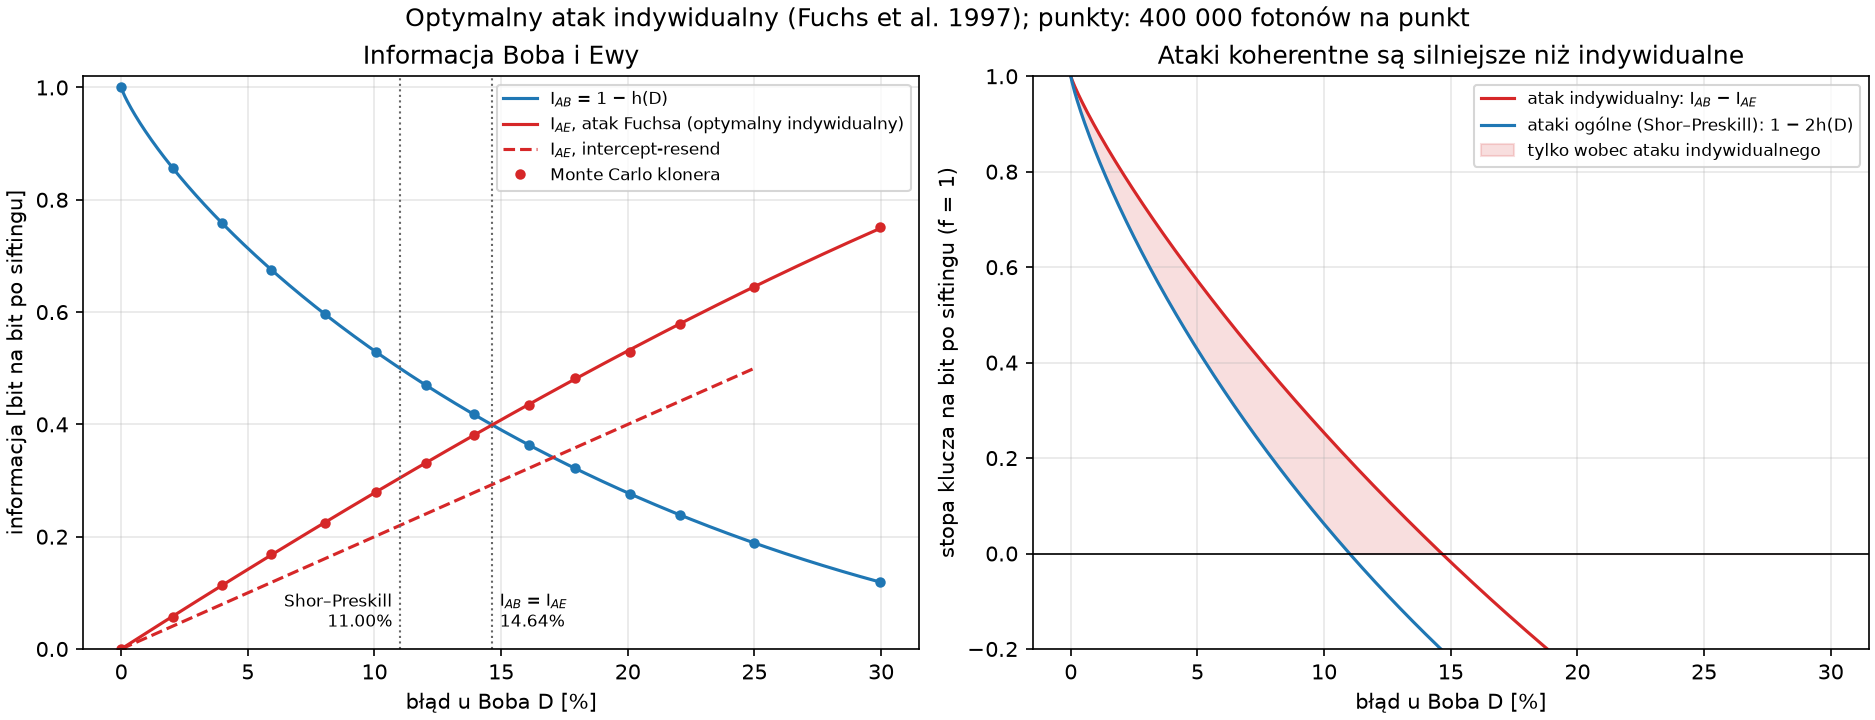
\includegraphics[width=\linewidth]{e08_individual_attack}
  \caption{Informacja Boba i Ewy w optymalnym ataku indywidualnym (linie: wzór Fuchsa, punkty: Monte Carlo), próg Shora--Preskilla i punkt intercept-resend.}
  \label{fig:e08}
\end{figure}

\subsection{Man-in-the-middle}

Ewa przecina światłowód i prowadzi dwa niezależne BB84: z Alice, udając Boba, i z Bobem, udając Alice. Fizyka nie ma czego wykryć: oba odcinki to uczciwe łącza z QBER jak bez ataku, a Ewa zna oba klucze. Obroną jest uwierzytelnianie Wegmana--Cartera \cite{wegman1981new}: tag $(h_k(m) + r) \bmod p$ z haszem wielomianowym nad GF($p$), $p = 2^{61} - 1$, kluczem $k$ na sesję i świeżym kluczem jednorazowym $r$ na tag. Monte Carlo potwierdza p-stwo fałszerstwa $1/p$ dla krótkich tagów, a w symulacji protokół przerywa się przy pierwszym sprawdzanym tagu Ewy: przy jej pierwszej wiadomości albo, przy tagu na transkrypt, na końcu rundy, przed użyciem klucza. Tag na każdą wiadomość zużywa więcej klucza, niż QKD wytwarza (Cascade wysyła wiadomość na każdy poprawiany błąd), więc tagujemy transkrypt rundy: 122~bity klucza na rundę. Bilans jest dodatni do 60,5~km przy $10^6$ impulsów na rundę, 104,5~km przy $10^7$ i 132~km przy $10^8$: QKD rozszerza klucz, a nie tworzy go z niczego.

\section{Skończony klucz}

Rachunek asymptotyczny zakłada nieskończony blok. Dla bloku $n$ bitów klucza i $k$ bitów testu używamy twierdzenia Tomamichela i in.\ \cite{tomamichel2012tight}: protokół przerywa się, gdy QBER z próbki przekroczy próg $Q_{\mathrm{tol}}$ ustalony z góry, a długość klucza zależy od $Q_{\mathrm{tol}}$ i poprawki statystycznej, a nie od zmierzonego QBER. Stopa rośnie z $n$ w stronę granicy $1 - 2h(Q)$ (rys.~\ref{fig:e07}). Uproszczenie z planu projektu (nierówność Hoeffdinga na samej próbce) pomija przeniesienie błędu z próbki na klucz przy losowaniu bez zwracania i zawyża długość klucza o 95\% przy $n = 3000$ i o 15\% przy $n = 10^5$.

Uwaga: oba twierdzenia wydrukowane w artykule dają przy parametrach jego Tabeli~1 stopy niższe o 8--14\% niż sama tabela. Implementacja trzyma się wzorów, a rozbieżność zostaje otwarta.

,,Ewa w szumie'': przy QBER tła 2\% i próbce 1000 bitów przechwycenie 4\% impulsów wykrywa się tylko w 23\% sesji, a 8\% w 78\%. Mały atak ginie w fluktuacjach i to właśnie rachunek skończonego klucza wycenia go w długości klucza.

\begin{figure}[t]
  \centering
  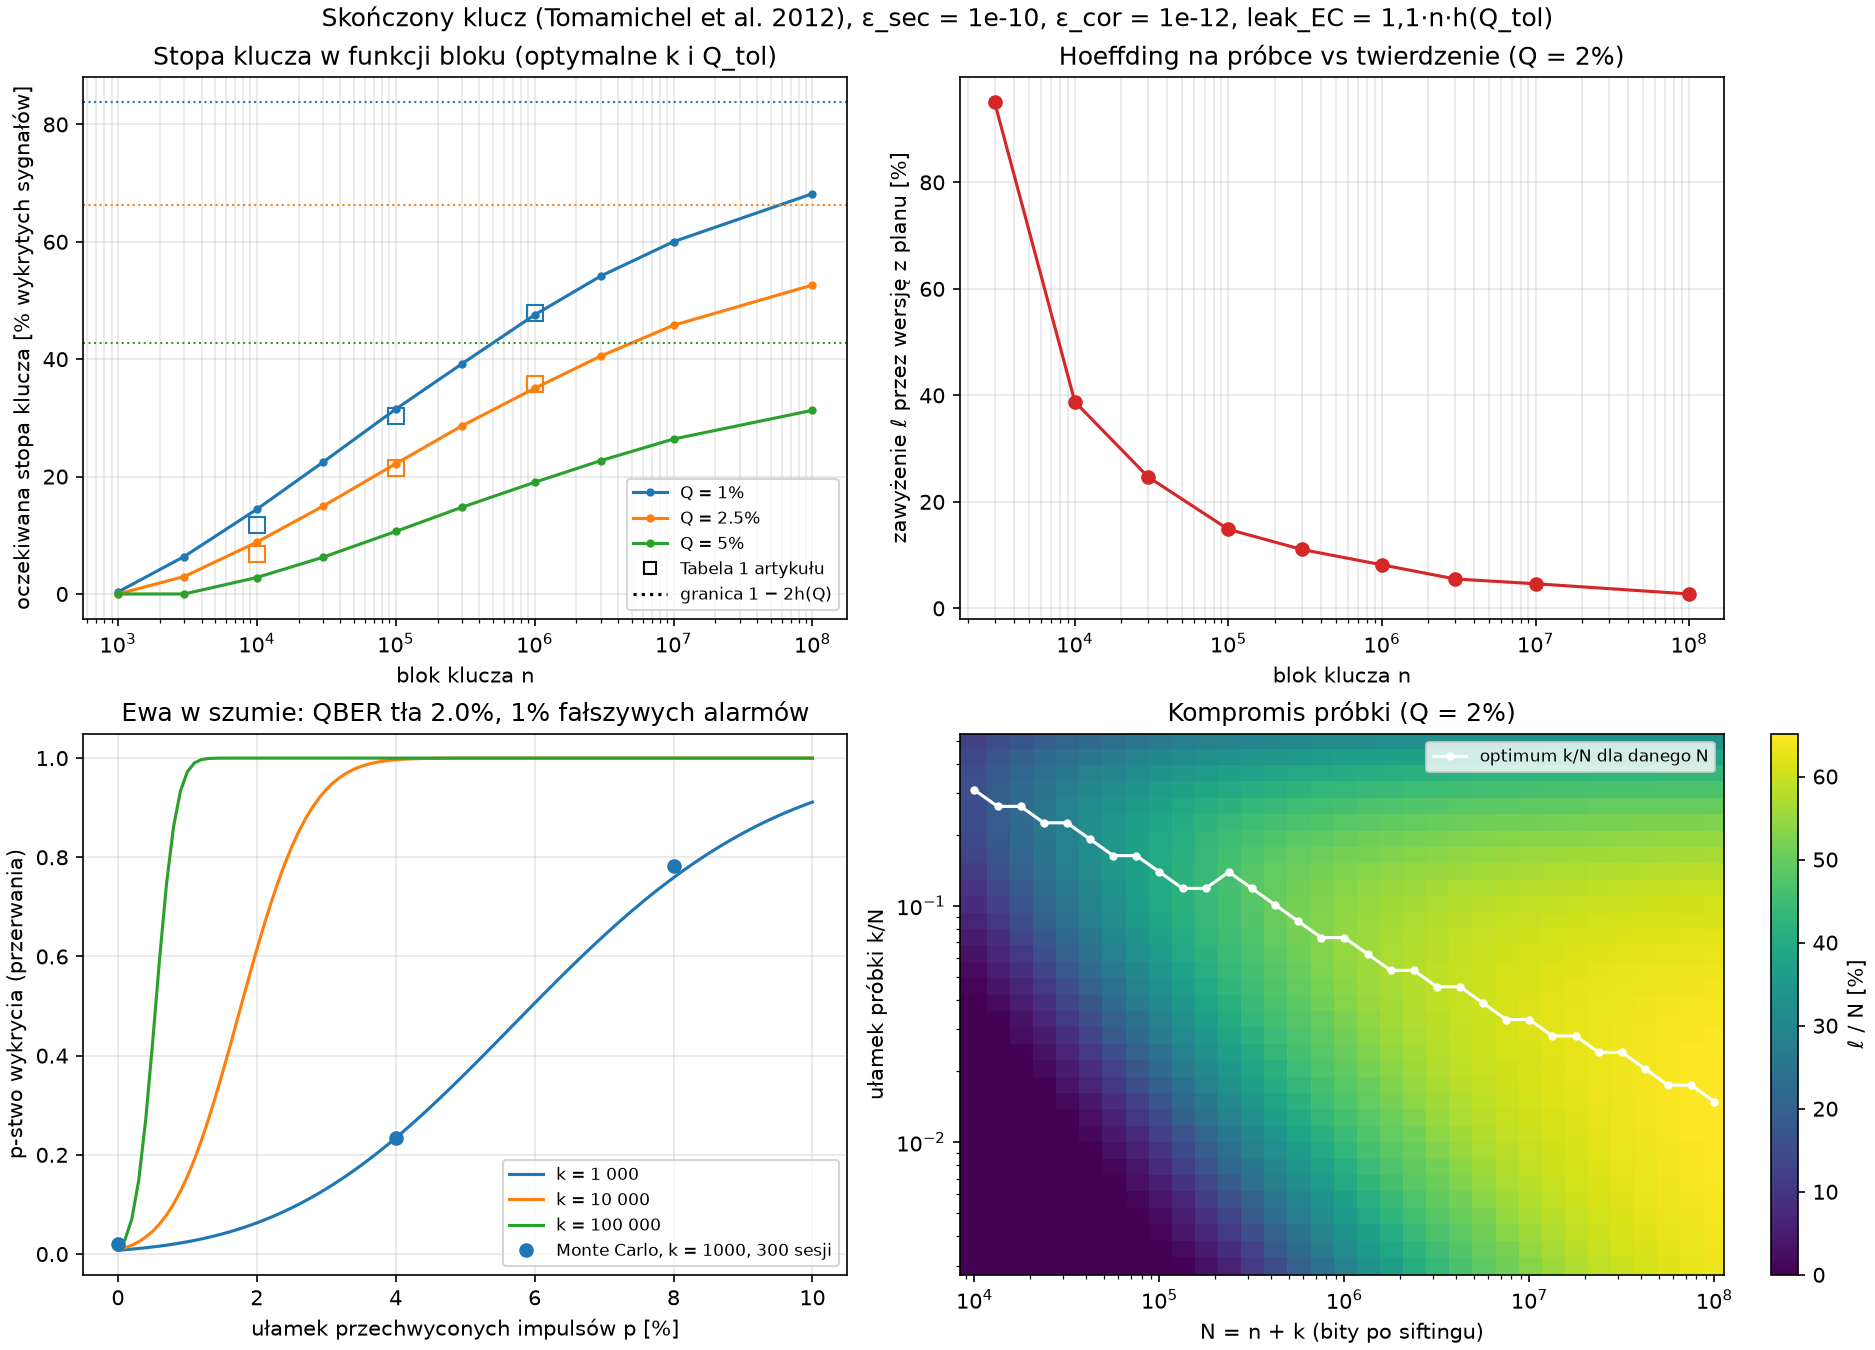
\includegraphics[width=0.75\linewidth]{e07_finite_key}
  \caption{Skończony klucz: stopa w funkcji bloku $n$ dla kilku QBER (Tomamichel i in.), zawyżenie przez uproszczenie Hoeffdinga, p-stwo wykrycia częściowego intercept-resend (,,Ewa w szumie'') oraz kompromis między wielkością próbki a długością klucza.}
  \label{fig:e07}
\end{figure}

\section{QKD a kryptografia postkwantowa}

\subsection{Uwierzytelnianie kanału klasycznego}

QKD potrzebuje uwierzytelnionego kanału klasycznego, ale tylko \emph{w trakcie} sesji: złamanie uwierzytelnienia później nie odsłania klucza, bo klucz zależy wyłącznie od tego, co Ewa podsłuchała. Wegman--Carter daje to bezwarunkowo, ale zużywa klucz. Alternatywą jest podpis postkwantowy ML-DSA \cite{nist2024fips204}, który nie zużywa klucza, za cenę założenia obliczeniowego, które musi stać w czasie sesji.

Każda strona podpisuje swój transkrypt rundy. Używamy ML-DSA z biblioteki \texttt{cryptography} (OpenSSL), a zgodność z niezależną implementacją \texttt{dilithium-py} sprawdzamy w obie strony dla poziomów 44, 65 i 87. Klucze publiczne są rozprowadzone z góry, bez PKI. Tabela~\ref{tab:mitm} zbiera scenariusze ataku MITM; wszystkie dają przewidywany wynik.

\begin{table}[t]
  \centering
  \caption{Scenariusze MITM (GYS, Ewa w połowie 25~km, $2\cdot 10^6$ impulsów na sesję). ,,Wykryty'' oznacza przerwanie protokołu przy sprawdzeniu transkryptu Ewy.}
  \label{tab:mitm}
  \small
  \begin{tabularx}{\linewidth}{>{\raggedright\arraybackslash}p{6.2cm} L}
    \toprule
    Scenariusz & Wynik \\
    \midrule
    (a) bez uwierzytelniania & MITM udany, QBER jak bez ataku \\
    (b) Wegman--Carter & wykryty \\
    (c) ML-DSA-65 & wykryty \\
    (d) ML-DSA złamane w trakcie sesji (wyrocznia fałszerstw) & MITM udany \\
    (e) ML-DSA złamane po sesji & Ewa zna 0 z 5662 bitów klucza \\
    (f) klucz Ewy w katalogu ofiary & MITM udany mimo ML-DSA \\
    (g) hybryda WC + ML-DSA, ML-DSA złamane w trakcie & wykryty \\
    \midrule
    ML-KEM-768 złamane po sesji (HNDL) & Ewa odzyskuje 256 z 256 bitów sekretu \\
    KDF(klucz QKD $\|$ sekret ML-KEM), HNDL & Ewa nie zna klucza wynikowego \\
    \bottomrule
  \end{tabularx}
\end{table}

Scenariusz (e) to tzw.\ \emph{everlasting security}: po wycieku kluczy prywatnych ML-DSA Ewa może podpisywać przyszłe sesje, ale o kluczu z tej sesji wie tyle, ile wynika z transkryptu. Liniowa Ewa z sekcji~2.2 liczy to dokładnie: transkrypt ujawnia 2605 niezależnych funkcji klucza przed wzmacnianiem prywatności i żadnej funkcji klucza końcowego. Dla kontrastu nagrany szyfrogram ML-KEM \cite{nist2024fips203} po przyszłym złamaniu krat oddaje cały sekret (,,harvest now, decrypt later'').

\begin{figure}[t]
  \centering
  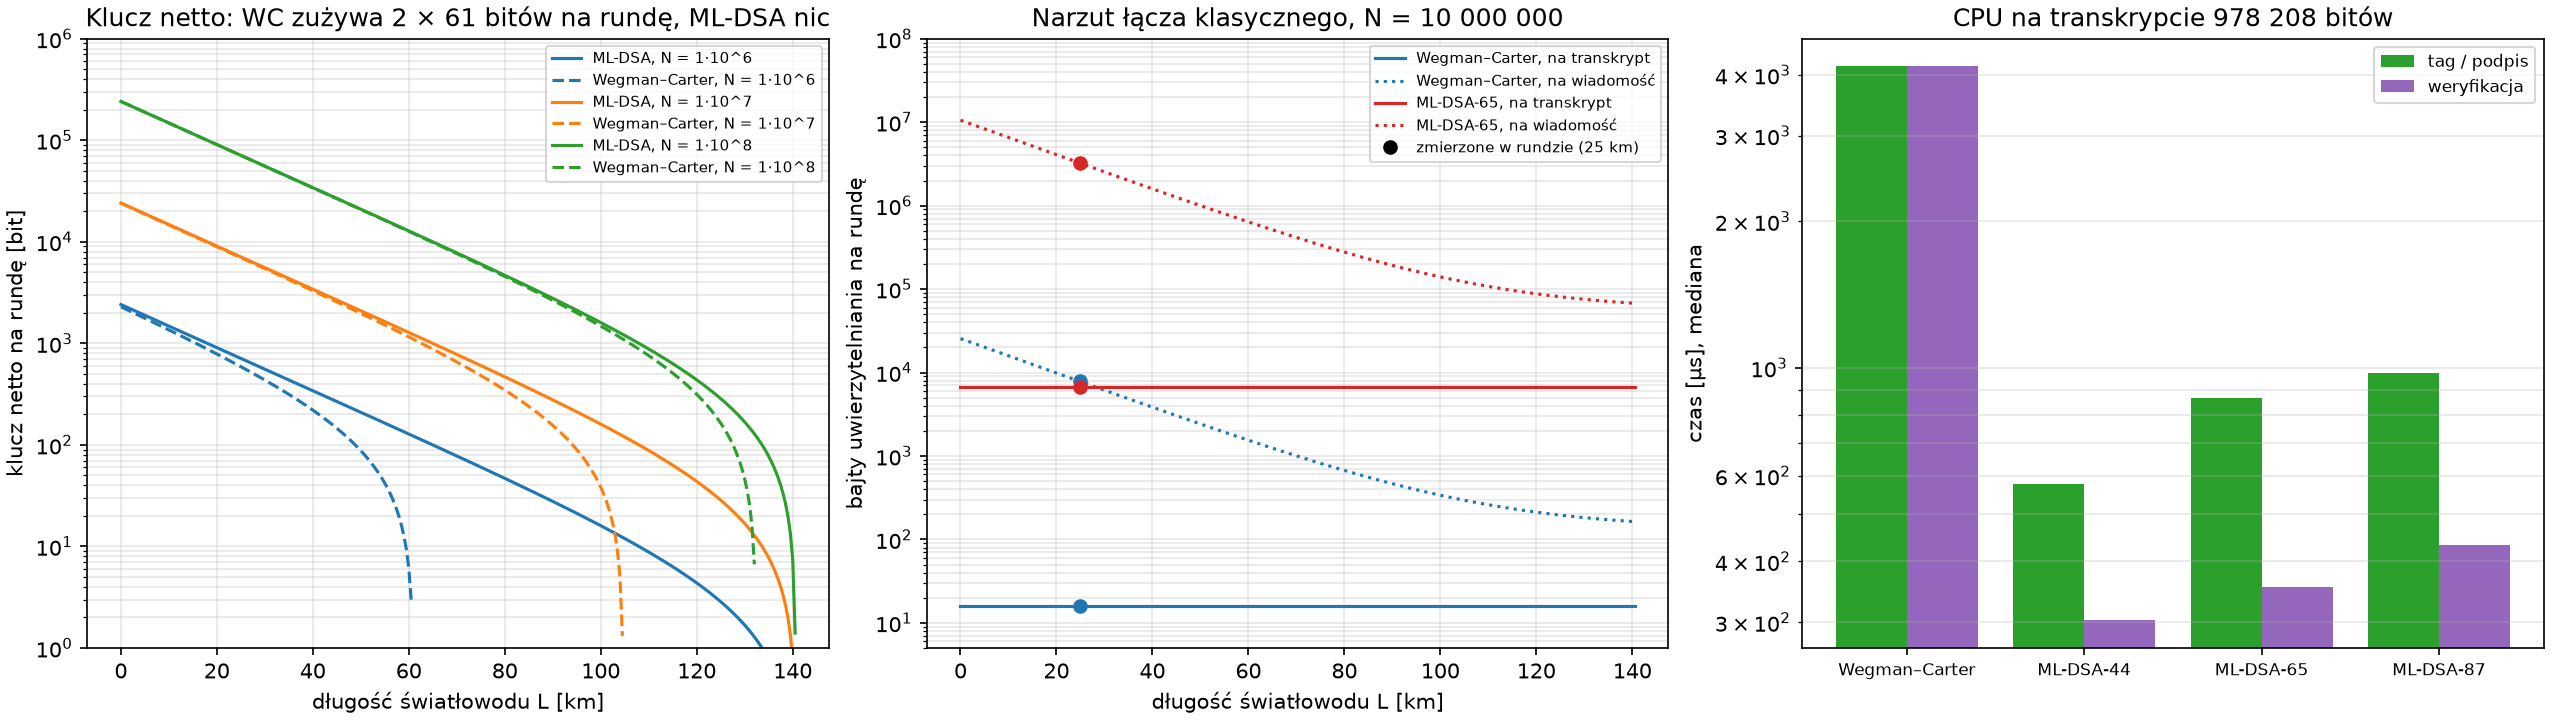
\includegraphics[width=\linewidth]{e10_pqc_auth}
  \caption{Uwierzytelnianie Wegmana--Cartera i ML-DSA. Lewy: klucz netto na rundę w funkcji L. Środek: bajty uwierzytelniania na rundę (linie: model, punkty: zmierzone przy 25~km). Prawy: czas tagu, podpisu i weryfikacji na transkrypcie rundy (hasz Wegmana--Cartera to pętla w Pythonie).}
  \label{fig:e10}
\end{figure}

Koszt (rys.~\ref{fig:e10}): ML-DSA-65 to 2 podpisy po 3309~B na rundę i około 2~ms CPU, a Wegman--Carter to 16~B i 122~bity klucza. Ponieważ ML-DSA nie zużywa klucza, bilans przy $10^6$ impulsów na rundę jest dodatni do 140,5~km zamiast 60,5~km. Podpis na każdą wiadomość kosztowałby 491 razy więcej bajtów (3,2~MB na rundę przy 25~km, więcej niż sam klucz) i kilkaset razy więcej czasu, a bezpieczeństwo byłoby takie samo, bo klucz powstaje dopiero po sprawdzeniu transkryptu. Rozmiary kluczy i podpisów zgadzają się z FIPS~204.

\subsection{Modele zagrożeń}

Tabela~\ref{tab:threats} porównuje trzy konstrukcje: QKD uwierzytelnione ML-DSA, ML-KEM oraz hybrydę, w której klucz to KDF z klucza QKD i sekretu ML-KEM (HKDF-SHA256). Nierówność Moski \cite{mosca2018cybersecurity} mówi, że dane są zagrożone, gdy czas, przez jaki mają pozostać tajne ($x$), plus czas migracji ($y$) przekracza czas do złamania ($z$). Dla QKD z uwierzytelnianiem $x$ dotyczy tylko podpisu i skraca się do długości sesji.

\begin{table}[t]
  \centering
  \caption{Modele zagrożeń. Wyniki liczbowe z e06 i e10.}
  \label{tab:threats}
  \small
  \begin{tabularx}{\linewidth}{>{\raggedright\arraybackslash}p{2.7cm} L L L}
    \toprule
    Zagrożenie & QKD + ML-DSA & ML-KEM-768 & Hybryda KDF \\
    \midrule
    Harvest now, decrypt later ($x + y > z$) & odporne: po wycieku klucza podpisu Ewa zna 0 bitów (e) & podatne: szyfrogram 1088~B i późniejsze złamanie dają cały sekret & odporne, dopóki tajny jest klucz QKD \\
    Przyszłe złamanie krat & przeszłe klucze bezpieczne; dalej Wegman--Carter z kluczem z QKD & wszystkie nagrane sesje odkryte & przeszłe klucze bezpieczne \\
    Złamanie podpisu w czasie rzeczywistym & MITM udany (d); z hybrydą WC + ML-DSA wykryty (g) & MITM udany: ML-KEM też wymaga uwierzytelnienia & bezpieczne, jeśli QKD uwierzytelnia hybryda (g) \\
    Ataki na implementację & sprzęt: oślepianie, time-shift, Trojan horse; obroną jest monitoring, a nie dowód & oprogramowanie: kanały boczne, np.\ KyberSlash \cite{bernstein2025kyberslash} & trzeba złamać obie implementacje \\
    Zasięg i infrastruktura & R(L) $> 0$ do około 140~km; osobny światłowód i detektory & bez limitu; 1184~B klucza publicznego i 1088~B szyfrogramu & ograniczenia QKD plus koszt ML-KEM \\
    Węzły pośrednie & dalej niż zasięg: węzły zaufane znają klucz & end-to-end & węzeł zna tylko składową QKD \\
    \bottomrule
  \end{tabularx}
\end{table}

Wniosek: QKD i ML-KEM chronią przed różnymi rzeczami. QKD daje bezpieczeństwo odporne na przyszłe złamanie, ale wymaga uwierzytelnienia w chwili sesji, osobnej infrastruktury i ma ograniczony zasięg; jego słabym punktem są urządzenia (sekcja~4). ML-KEM działa wszędzie, ale nagrany ruch jest bezpieczny tylko tak długo, jak założenia kratowe. Hybryda dziedziczy mocniejszą stronę każdej z nich w modelu HNDL i przy atakach na implementację, a słabości infrastrukturalne QKD.

\section{Ograniczenia i wnioski}

Model pomija dyspersję i dryf polaryzacji, a $e_d$ i $Y_0$ nie zależą od długości ani od czasu. Skończony klucz liczymy dla źródła jednofotonowego; wersja dla WCP z decoy \cite{lim2014concise} jest planowana w kolejnej wersji, podobnie jak ataki time-shift \cite{qi2007timeshift,zhao2008quantum}, Trojan horse \cite{gisin2006trojan,lucamarini2015practical} i słaby generator liczb losowych. Atak 6 działa na pojedynczych fotonach i idealnych detektorach, bo jest granicą teoretyczną. Scenariusze złamania ML-DSA są wyidealizowane (Ewa ma po prostu klucz prywatny), a kanałów bocznych implementacji PQC nie modelujemy. Czas CPU Wegmana--Cartera mierzymy na implementacji w Pythonie i nie jest on reprezentatywny dla metody.

Wnioski: (1) zwalidowany tor Monte Carlo odtwarza wartości kontrolne z literatury i z niezależnej implementacji; (2) wszystkie ataki, które nie podnoszą QBER (oślepianie, PNS, MITM), łamią założenie dowodu, a nie wzór na długość klucza, i każdy ma obronę z mierzalną metryką; (3) uwierzytelnianie podpisem postkwantowym zachowuje zaletę QKD wobec ,,harvest now, decrypt later'', o ile podpis wytrzymuje czas sesji, a hybryda z Wegmanem--Carterem usuwa nawet to założenie.

Kod, dane i wykresy: repozytorium projektu (\texttt{make figures}, \texttt{make report}).

\bibliographystyle{unsrt}
\bibliography{references}

\end{document}
